% Canonical caption for figSubjectPredictors.pdf
% Generated by: code/module_c/mc_figures.py from q2_primary.csv and
% q2_coefficients.csv in code/figures/module_c/cohorts_2014_2019/
\begin{figure}[p]
  \centering
  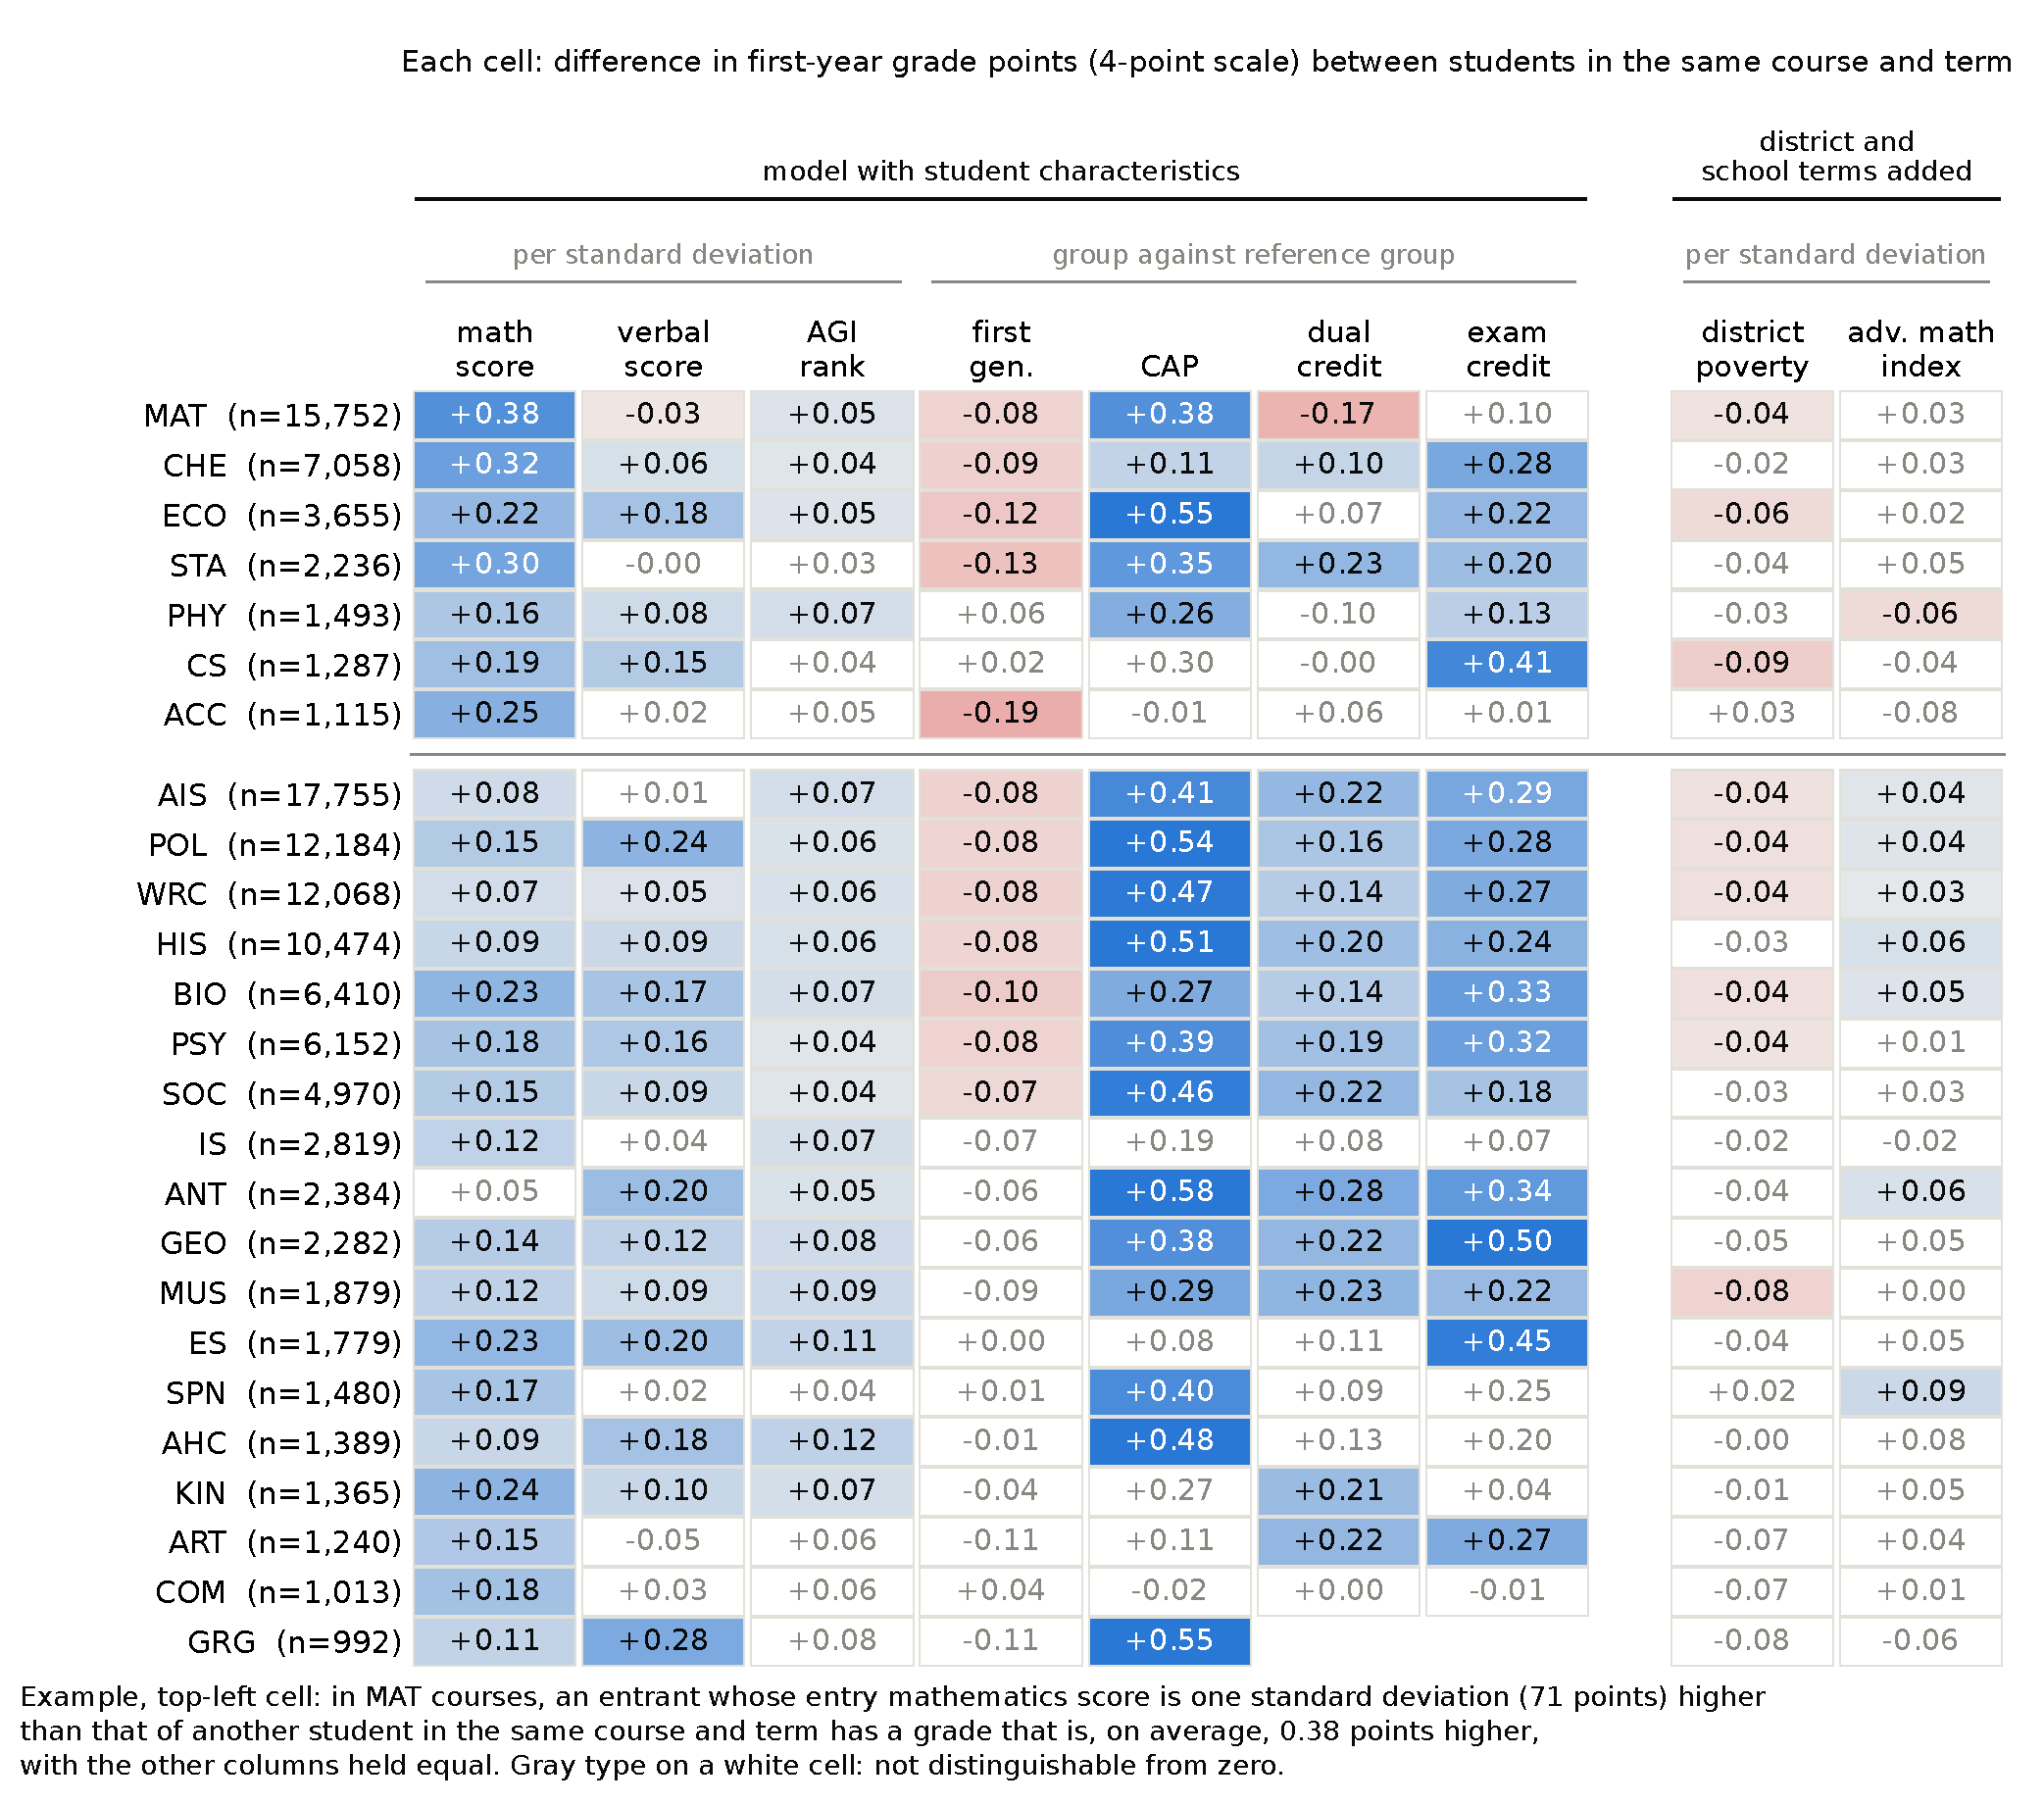
\includegraphics[width=0.80\textwidth]{figSubjectPredictors.pdf}
  \caption{Associations between entry characteristics and
    first-year grades in the 25 subjects in which at
    least 1,000 linked entrants of Fall 2014 to Fall 2018 hold a
    first attempt. Each subject has two regressions with
    course-by-term fixed effects, so students are compared within
    the same course and term: the first seven columns come from a
    model with student characteristics, and the last two from the
    same model with district and school terms added. Each cell is
    the difference in grade points (4-point scale) that goes with
    the column's characteristic, the other characteristics of its
    model held equal; the figure prints a worked example for the
    top-left cell (0.38 grade points is about a third of
    a letter grade). Columns marked per standard deviation give
    the difference that goes with one standard deviation of the
    characteristic. Columns marked group against reference
    compare first-generation entrants with entrants who are not
    first-generation, CAP entrants with other entrants, and
    entrants holding each type of pre-college mathematics credit
    with entrants holding none. A shaded cell (blue positive, red
    negative) has an interval that excludes zero: score columns
    under false-discovery control at $q=0.05$ across subjects,
    other columns at unadjusted $p<0.05$. The 7 quantitative
    subjects sit above the rule. The count $n$ is the number of
    linked entrants with a graded first attempt and can fall
    below the 1,000 that admit a subject (the smallest is
    992). Standard errors are clustered on sending school;
    every cell is an association conditional on entry.
    Subject codes: MAT, mathematics; CHE, chemistry; ECO, economics; STA, statistics; PHY, physics; CS, computer science; ACC, accounting; AIS, the first-year seminar; POL, political science; WRC, writing composition; HIS, history; BIO, biology; PSY, psychology; SOC, sociology; IS, information systems; ANT, anthropology; GEO, geology; MUS, music; ES, environmental science; SPN, Spanish; AHC, art history and criticism; KIN, kinesiology; ART, art; COM, communication; GRG, geography.}
  \label{figSubjectPredictors}
\end{figure}
